\documentclass{webofc}
\usepackage[varg]{txfonts}   % Web of Conferences font
%
% Put here some packages required or/and some personnal commands
%
\usepackage{hyperref}
\hypersetup{colorlinks=false}

%
\begin{document}
%
\title{IPv6-only networking on WLCG}
%
% subtitle is optionnal
%
%%%\subtitle{Do you have a subtitle?\\ If so, write it here}

\author{
  \firstname{Marian} \lastname{Babik}\inst{1}\and
  \firstname{Martin} \lastname{Bly}\inst{2}\and
  \firstname{Nick} \lastname{Buraglio}\inst{3}\and
  \firstname{Tim} \lastname{Chown}\inst{4}\and
  \firstname{Dimitrios} \lastname{Christidis}\inst{1}\and
  \firstname{Ji\v{r}i} \lastname{Chudoba}\inst{5}\and
  \firstname{Phil} \lastname{DeMar}\inst{6}\and
  \firstname{Jos\'e} \lastname{Flix~Molina}\inst{7}\and
  \firstname{Costin} \lastname{Grigoras}\inst{1}\and
  \firstname{Bruno} \lastname{Hoeft}\inst{8}\and
  \firstname{Hiro} \lastname{Ito}\inst{9}\and
  \firstname{David} \lastname{Kelsey}\inst{2}\thanks{\email{david.kelsey@stfc.ac.uk}} \and
  \firstname{Edoardo} \lastname{Martelli}\inst{1}\and
  \firstname{Shawn} \lastname{McKee}\inst{10}\and
  \firstname{Maria del Carmen} \lastname{Misa~Moreira}\inst{1}\and
  \firstname{Raja} \lastname{Nandakumar}\inst{2}\and
  \firstname{Kars} \lastname{Ohrenberg}\inst{11}\and
  \firstname{Francesco} \lastname{Prelz}\inst{12}\and
  \firstname{Duncan} \lastname{Rand}\inst{13}\and
  \firstname{Andrea} \lastname{Sciab\`a}\inst{1}\and
  \firstname{Tim} \lastname{Skirvin}\inst{6}
}

\institute{ 
  European Organization for Nuclear Research (CERN), CH-1211 Geneva 23, Switzerland
\and
  UKRI STFC Rutherford Appleton Laboratory (RAL), Harwell Campus, Didcot OX11 0QX, United Kingdom
\and
  Energy Sciences Network (ESNET), Lawrence Berkeley National Laboratory, 1 Cyclotron Rd, Berkeley CA 94720, United States of America
\and
  JISC, Lumen House, Library Avenue, Harwell Campus, Didcot OX11 0SG, United Kingdom
\and
  Institute of Physics, Academy of Sciences of the Czech Republic, Na Slovance 2 182 21 Prague 8, Czech Republic
\and
  Fermi National Accelerator Laboratory (FNAL), P.O. Box 500, Batavia IL 60510, United States of America
\and
  Centro de Investigaciones Energ\'eticas, Medioambientales y Tecnol\'ogicas (CIEMAT), Av. Complutense 40, E-28040 Madrid, Spain
\and
  Karlsruhe Institute of Technology (KIT), Hermann-von-Helmholtz-Platz 1, D-76344 Eggenstein-Leopoldshafen, Germany 
\and
  Brookhaven National Laboratory (BNL), 98 Rochester St., Upton NY 11973, United States of America
\and
  University of Michigan, 500 S State S, Ann Arbor MI 48109, United States of America
\and
  Deutsches Elektronen-Synchrotron (DESY), Notkestra\ss e 85, D-22607 Hamburg, Germany
\and
  INFN, Sezione di Milano, via G. Celoria 16, I-20133 Milano, Italy
\and
  Imperial College London, South Kensington Campus, London SW7 2AZ, United Kingdom
}

\abstract
{The transition of WLCG storage services to dual-stack IPv4/IPv6 is nearing completion after more
than 5 years, thus enabling the use of IPv6-only CPU resources as agreed by the WLCG Management
Board and presented by us at earlier CHEP conferences. Much of the data is transferred by the LHC
experiments over IPv6. All Tier-1 storage and over 90% of Tier-2 storage is now IPv6-enabled, yet we
still see IPv4 transfers happening when both endpoints have IPv6 available or when remote data is
accessed over the network from worker nodes.
The monitoring and tracking of all data transfers is essential, together with the ability to understand
the relative use of IPv6 and IPv4. This paper presents the status of monitoring IPv6 data flows within
WLCG and plans to improve the ability to distinguish between IPv6 and IPv4. Furthermore, the
Research Networking Technical Working Group has identified marking the IPv6 packet header as one
approach for understanding complex large data flows. This provides another driver for a full
transition to the use of IPv6 in WLCG data transfers.
The agreed endpoint of the WLCG transition to IPv6 remains the deployment of IPv6-only services,
thereby removing the complexity and security concerns of operating dual stacks. The working group
is identifying where IPv4 can be removed and investigating the obstacles to the use of IPv6 in WLCG.
Why do transfers between two dual-stack endpoints still use IPv4? This work is presented together
with the obstacles defeated, those remaining, and those outside of our control.}
\maketitle
\section{Introduction}
\label{sec-intro}
%section 1

The HEPiX IPv6 Working Group \cite{ipv6wg} has been investigating the many issues involved in the deployment and use of
IPv6 in HEP in general and more specifically in WLCG. The group's paper at CHEP2016 \cite{ipv6chep2016}
presented the status then of the work to allow sites to deploy IPv6-only CPU resources. Driven by the
requirements of the LHC experiments, the WLCG Management Board, in September 2016, had approved our plan
that all WLCG Tier-2 storage services should aim to support dual-stack IPv6/IPv4 by the end of 2018. Since then the
group has worked with others to encourage, support and monitor that transition and to identify and help
solve any technical issues as they arise.

%This paper is organised as follows.  Section 2 presents the current status of the transition for the Tier0/Tier1s, the Tier2s and the Experiment Services.
%Section 3 presents an update on service availability and network monitoring and also reports on the fraction of FTS data transfers currently taking place over IPv6.
%Finally section 4 contains future plans and conclusions. 

 

%
\section{Status of the IPv4/IPv6 dual-stack transition at WLCG sites}
\label{sec-dualstack}
%section 2 - Status of the IPv4/IPv6 dual-stack transition at WLCG sites


%
\section{Obstacles in the transition to IPv6}
\label{sec-obstacles}
In the practical, day-to-day experience of fostering the transition to
the prevalent usage of IPv6 at WLCG sites our group observed many obstacles.
A significant number of these were addressed and eventually overcome. We
find it valuable to record this experience not just to help similar
processes in other organisations but also to keep the momentum for tackling
the last remaining hurdles.
%
\subsection{IPv6 obstacles that were identified}
\label{sec-obstacles-found}
%section 3.1 IPv6 obstacles that were identified

Several obstacles have being delaying the deployment of IPv6 and identifying them has been an important task of the Working Group.
These are the main obstacles that we have been addressing:
\begin{itemize}
  \item Applications don't support or understand IPv6
  \item WLCG Sites not yet deployed IPv6 networking
  \item Sites have IPv6 but Tier-2 has no dual-stack storage
  \item IPv6 monitoring not available or broken
  \item Service is dual-stack but IPv4 being used
\end{itemize}

Support for IPv6 in WLCG application was one of the first obstacles tackled by the Working Group. Applications were first tested on a dual-stack environment and problems were reported to the developers. We maintained a list of the applications with indication of their IPv6 compliance or not. It took a long time, but most of the incompatibility have been removed and today the most important applications work properly with IPv6.

Lack of IPv6 deployment at the sites has been another major obstacle. Deploying IPv6 is relatively easy in a small site, but deploying it at production level in a large site with all the IPv4 functionalities (DNS, firewalling, address management..) is a large and expensive task. Luckily the management of some large site understood the risk of delaying this deployment and made dual-stack networks a reality in several large sites.

But even when sites had IPv6 capable networks, IPv6 traffic was lacking. We soon realized that the most important service to give IPv6 capabilities was storage, so the Working Group proposed to WLCG to mandate the deployment of dual-stack storage. WLCG accepted and we started a GGUS ticket campaign asking every site to report on their progresses.
The campaign is still on-going, but luckily a critical mass was reached quickly and today more than 90% of the LHCOPN traffic is IPv6.

Now that IPv6 was flowing, we soon realized that in many situations it was not possible to measure it. Being storage the main source of network traffic, we have worked with the FTS developers to make it possible to distinguish the IP protocol used for the file transfers. Figure\ref{fig:fts-ipv6} shows a FTS monitoring dashboard in which is visible the moment FTS started distinguishing IPv6 from IPv4.
Other work was done on network monitoring, to distinguish the traffic by protocol on the main network link. In LHCOPN first we used the sflow data generated by the CERN routers, but  once they were replaced to support 400Gbps links, the sflow data became unreliable. So More work was done to separate IPv4 and IPv6 in different VLANs on all the LHCOPN routers.

\begin{figure}[h]
\centering
        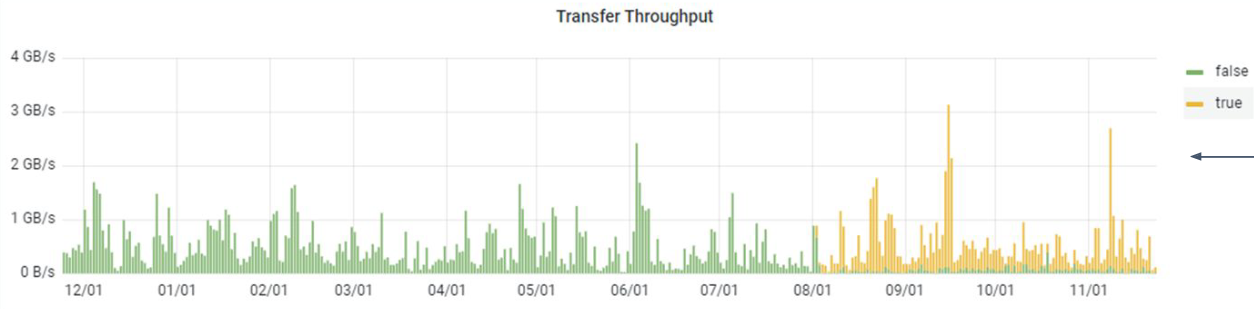
\includegraphics[width=\linewidth]{fts-ipv6.png}
\caption{FTS monitoring now able to distinguish IPv6 from IPv4}
\label{fig:fts-ipv6}
\end{figure}

Another subtle obstacle encountered was that although all the pieces were in place (dual-stack network, software IPv6 capable, service DNS names with correct AAAA records) clients were still preferring IPv4. In most cases it was some hidden or forgotten setting inside the application that forced the use of IPv4.
As an example, figure\ref{fig:aglt2-ipv6} shows  data transfers into USA/ATLAS Great Lakes Tier 2 (AGTL2) where it is possible to see the moment the
variable java.net.preferIPv6Addresses in dCache was set to true.

\begin{figure}[h]
\centering
        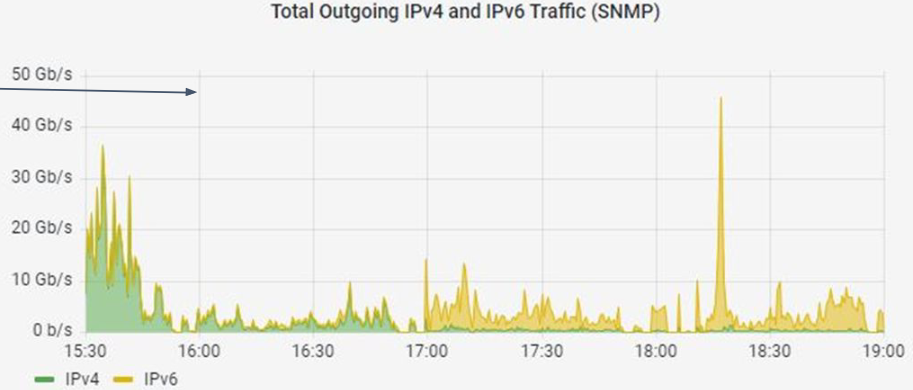
\includegraphics[width=\linewidth]{aglt2-ipv6.png}
\caption{Data transfers into USA/ATLAS Great Lakes Tier 2 (AGTL2)}
\label{fig:aglt2-ipv6}
\end{figure}

%%%% Is the rest part of this section???  %%%%%%%%%%%%%

Obstacles to IPv6 - to be addressed
5. Non-storage services not yet dual-stack
   a. ~60% of all WLCG services are dual-stack today
6. WLCG client CPU (worker nodes, VMs, containers) some IPv4-only
7. Services/clients outside of WLCG Tier-1/Tier-2 not yet considered
   a. Tier-3, Public/Commercial Clouds, Analysis facilities, Experiment portals…
8. Use of new or evolving technologies not yet tested or tracked
   a. New CPU architectures (GPU, non-x86, …), container orchestration, …
9. “People” can be the obstacle
   a. they do not consider use of IPv6 or refuse to deploy!



\subsection{IPv6 obstacles that were overcome}
\label{sec-obstacles-fixed}
%section 3.2 IPv6 obstacles that were overcome


\subsection{Remaining IPv6 obstacles}
\label{sec-obstacles-left}
%section 3.3 Remaining IPv6 obstacles


%
\subsection{Summary and future outlook}
\label{sec-future}
%section 4
\subsection{Obstacles and potential show-stoppers}
Our experience with the transition of WLCG Tier-1 and Tier-2 centers so far 
has identified various cases where the IPv4$\rightarrow$IPv6 transition has
consequences that exceed the simple replacement of the IP {\it transport} layer.
These broadly fall in the following categories:
\begin{enumerate}
\item Software components and protocol with fixed-size storage for network
addresses, for example in (Grid-)FTP and AFS. This can be overcome by appropriate
protocol extensions (e.g. the introduction of 'extended' FTP commands
{\tt EPRT}, {\tt EPSV}, etc.), with a large development effort required.
In certain cases (AFS) this effort was determined to be too large and not
worthwhile, while the GrifFTP 'v2' extensions were issued with no IPv6 support.
\item Software components and protocols that assume single addresses or a single
IP protocol for 
network endpoints (to various extents, all the components in the WLCG software
matrix). While all Operating Systems do provide hybrid network stacks and prioritized/configurable
source and destination address selection\footnote{Address selection is regulated in most cases by RFC6724.}, applications should always iterate over multiple
possible results (belonging to multiple IP protocol versions) and provide configurable
overrides and preferences. 
\item Software components and network infrastructures providing asymmetric
handling, or separate code stacks, for IPv4 and IPv6 traffic: these also
have the ability to load the network transport choice with measurable
performance consequences.
\end{enumerate}
Detecting and explaining these IPv4/IPv6 asymmetries and fostering improved
symmetry across the WLCG software matrix has been a long-standing activity
for our group. As there is inherent risk in changing, testing and rolling
out (sometimes sizable) software changes when no functional
issue requires immediate attention, these changes are often not shortlisted
for deployment by software development teams. We need to continue tracking
these issues down to the
level where no deployment of measurable performance asymmetry between the two
protocols is seen: this can be seen as the backdrop of any future activity.

\subsection{Further steps}
Once the data transfer monitoring infrastructure described in Section
\ref{sec-monitoring} is completed and covers all services, two cases
need to be consistently monitored and, where needed, investigated
and resolved:
\begin{enumerate}
\item cases where the fraction of data transferred over IPv6 is lower than expected:
the preference for IPv6 over IPv4 has to established throughout the system;
\item cases where the transfer performance is either significantly worse 
or significantly better on IPv6 over IPv4: asymmetries in the routing and
transport should be identified, especially in the LHCONE and LHCOPN networks.
\end{enumerate}
\par
Over a stable and understood data transfer network 
IPv6-only worker nodes should encounter no more operational anomalies
than other types of worker nodes. The 
job failure rate on IPV6-only, dual-stack and IPv4-only worker nodes should
be monitored statistically and deviations properly troubleshot.
\par
Once the use-case of IPv6-only worker nodes operates smoothly, the next
step in the transition roadmap is moving services and network segments to
IPv6-only operation.

\subsection{IPv6-only scenarios}
The final step of the IPv4$\rightarrow$IPv6 transition is the phasing out of
IPv4. While still in the non-near future, this is also arguably the only step
that can bring along a desirable reduction
in the infrastructure maintenance effort, so it shouldn't be delayed
without reason. Many of the issues described in the previous sections 
actually arise
from the fact that in the current transition phase many components and
configurations have to be maintained in parallel.
\par
In order to demonstrate that the close of the transition is a realistic
objective, IPv6-only operation of an entire WLCG Tier-X site will
need to have been proven by all experiments and sites run by most WLCG
partners, with residual IPv4-only services either deprecated or made
accessible via protocol translation techniques (e.g. DNS64/NAT64, see
NAT64/DNS64 (RFC6146/6147 \cite{rfc})). 
\par
%{\it XXX Should we mention the few experiments performed so far here ?}

\subsection{Conclusion}
The aim of allowing the successful execution of generic WLCG job payloads
on IPv6-only worker nodes has been driving the IPv4-IPv6 dual-stack deployment
of storage services across the WLCG production infrastructure. According to
the current progress tracking, summarised in Sections \ref{ssec-t1trans} and
\ref{ssec-t2trans} above, this step should be completed at CERN, Tier-1
and Tier-2 centres by the end of 2018. A few residual
issues were identified in the software stack in this process.
\par
Data from
a complete and pervasive monitoring infrastructure are crucial in building
confidence in the new transport layer, which is expected to provide the
{\it same} level of performance and reliability as the one it replaces: these
come from various sources (see Section \ref{sec-monitoring}), with a few
remaining blind spots being covered.
\par
Feedback from the actual operation of  
IPv6-only computing farms will then determine the time-scale and viability of
driving the transition process to its natural ending, when the burden
of operating a duplicated transport infrastructure will be eventually lifted.


% Etc. etc. etc.
%For one-column wide figures use syntax of figure~\ref{fig-1}
%\begin{figure}[h]
%% Use the relevant command for your figure-insertion program
%% to insert the figure file.
%\centering
%\includegraphics[width=1cm,clip]{tiger}
%\caption{Please write your figure caption here}
%\label{fig-1}       % Give a unique label
%\end{figure}
%
%For two-column wide figures use syntax of figure~\ref{fig-2}
%\begin{figure*}
%\centering
%% Use the relevant command for your figure-insertion program
%% to insert the figure file. See example above.
%% If not, use
%\vspace*{5cm}       % Give the correct figure height in cm
%\caption{Please write your figure caption here}
%\label{fig-2}       % Give a unique label
%\end{figure*}
%
%For figure with sidecaption legend use syntax of figure
%\begin{figure}
%% Use the relevant command for your figure-insertion program
%% to insert the figure file.
%\centering
%\sidecaption
%\includegraphics[width=5cm,clip]{tiger}
%\caption{Please write your figure caption here}
%\label{fig-3}       % Give a unique label
%\end{figure}
%
%For tables use syntax in table~\ref{tab-1}.
%\begin{table}
%\centering
%\caption{Please write your table caption here}
%\label{tab-1}       % Give a unique label
%% For LaTeX tables you can use
%\begin{tabular}{lll}
%\hline
%first & second & third  \\\hline
%number & number & number \\
%number & number & number \\\hline
%\end{tabular}
%% Or use
%\vspace*{5cm}  % with the correct table height
%\end{table}
%
% BibTeX or Biber users please use (the style is already called in the class, ensure that the "woc.bst" style is in your local directory)
% \bibliography{name or your bibliography database}
%
% Non-BibTeX users please use
%
%\begin{thebibliography}{}
%
% and use \bibitem to create references.
%
%\bibitem{rfc} All Internet Engineering Task Force Requests For Comments (RFC) do
%cuments are available
%from URLs such as http://www.ietf.org/rfc/rfcNNNN.txt where NNNN is the RFC numb
%er, for example {\tt http://www.ietf.org/rfc/rfc2460.txt}
% Format for Journal Reference
%Journal Author, Journal \textbf{Volume}, page numbers (year)
% Format for books
%\bibitem{RefB}
%Book Author, \textit{Book title} (Publisher, place, year) page numbers
% etc
%\end{thebibliography}
%
\begin{thebibliography}{}
%
% and use \bibitem to create references.
%
% Format for Journal Reference
%Journal Author, Journal \textbf{Volume}, page numbers (year)
% Format for books
%\bibitem{RefB}
%Book Author, \textit{Book title} (Publisher, place, year) page numbers
% etc


%section 1 references
%\bibitem{ipv6wg} The HEPiX IPv6 Working Group, http://hepix-ipv6.web.cern.ch
\bibitem{ipv6wg}
S. Campana et al, J. Phys. Conf. Ser. {\bf513}, 062026 (2014)



%\bibitem{ipv6chep2016} 
% M. Babik et al, J. Phys. Conf. Ser. {\bf898}, 082033 (2017)
\bibitem{ipv6chep2018} 
M. Babik et al, J. Phys. Conf. Ser. {\bf214}, 08010 (2019)

\bibitem{eos} A. J. Peters et al, J. Phys. Conf. Ser. {\bf664}, 042042 (2015)


%section 2 references

\bibitem{rfc} 
All Internet Engineering Task Force Requests For Comments (RFC) documents are available
from URLs such as https://www.ietf.org/rfc/rfcNNNN.txt where NNNN is the RFC number, for example {\tt https://www.ietf.org/rfc/rfc2460.txt}



%section 2 intro para

\bibitem{ipv6chep2015} 
J. Bernier et al, J. Phys. Conf. Ser. {\bf664}, 052018 (2015)

%section 2.1 Tier 0/1
\bibitem{fts3}
A.~A. Ayllon et al, 
%M~Salichos, M~K Simon, and O~Keeble.
%\newblock Fts3: New data movement service for wlcg.
J. Phys. Conf. Ser. {\bf 513}, 032081 (2014)

%section 2.2 Tier 2

%section 2.3 LHCOPN
\bibitem{opnone}
E. Martelli et al, J. Phys. Conf. Ser. {\bf 664}, 052025 (2015)

%section 2.4 Data transfers



%section 2 Experiments
%\bibitem{alien} 
%S. Bagnasco et al, J. Phys. Conf. Ser. {\bf119(6)}, 062012 (2008)

%\bibitem{xrootd}
%L. Bauerdick et al, J. Phys. Conf. Ser. {\bf 396} 042009 (2012)

%\bibitem{jalien}
%A. Grigora et al, J. Phys. Conf. Ser. {\bf523}, 012010 (2014)

%\bibitem{glideinwms} 
%http://iopscience.iop.org/article/10.1088/1742-6596/119/6/062044
%I. Sfiligoi, J. Phys. Conf. Ser. {\bf119(6)}, 062044 (2008)

%\bibitem{htcondor}
%D. Thain et al, Concurrency - Practice and Experience, {\bf 7(2-4)}, 323 (2005)

%\bibitem{dirac} A. Tsaregorodtsev et al, J. Phys. Conf. Ser. {\bf513}, 032096 (2014)

%LHCb : LHCb collaboration, A. A. Alves Jr. et al., The LHCb detector at the LHC, JINST 3 (2008) S08005

%section 3 references

%section 3.1
\bibitem{ipv6trans}
M. Nikkhah and R. Gu\'erin, 
IEEE/ACM Transactions on Networking, {\bf 24(4)}, 2291 (2016)

\bibitem{jool}
https://www.jool.mx

%section 3.2

\bibitem{RefLHCOPNEv4v6}
LHCOPN and LHCONE traffic flows on the CERN border routers, 
https://twiki.cern.ch/twiki/bin/view/LHCOPN/LHCOPNEv4v6Traffic


%section 3.3
\bibitem{frontier}
http://frontier.cern.ch/

%\bibitem{sam}
%A. Aimar et al, J. Phys. Conf. Ser. {\bf 898(9)}, 092033 (2017)
%A~Aguado Corman, P~Andrade, S~Belov, J~Delgado Fernandez, B~Garrido Bear, M~Georgiou, E~Karavakis, L~Magnoni, R~Rama Ballesteros, H~Riahi, J~Rodriguez Martinez, P~Saiz, and D~Zolnai.
%\newblock Unified monitoring architecture for it and grid services.


%\bibitem{etf}
%Marian Babik, CERN,
%\newblock Experiments {Test} {Framework} ({ETF}).
%http://etf.cern.ch/docs/latest/

%\bibitem{perfsonar} 
%A. Hanemann et al, 
%Jeff~W. Boote, Eric~L. Boyd, J{\'e}r{\^o}me Durand, Loukik
 %Kudarimoti, Roman {\L}apacz, D.~Martin Swany, Szymon Trocha, and Jason Zurawski.
%\newblock Perfsonar: A service oriented architecture for multi-domain network monitoring.
%\newblock In Boualem Benatallah, Fabio Casati, and Paolo Traverso, editors,
  %{\em Service-Oriented Computing - ICSOC 2005}, pages 241--254, Berlin, Heidelberg, 2005. Springer Berlin Heidelberg.

%\bibitem{wlcg-NTWG}
%S.~McKee et al, J. Phys. Conf. Ser. {\bf 664(5)} 052003 (2015)
%S.~Campana, A.~Di Girolamo, T.~Wildish, J.~Closier, S.~Roiser, C.~Grigoras, I.~Vukotic, M.~Salichos, Kaushik De, V.~Garonne, J.A.D. Cruz, A.~Forti, C.J. Walker, D.~Rand, A.~de~Salvo, E.~Mazzoni, I.~Gable, F.~Chollet, L.~Caillat, F.~Schaer, Hsin-Yen Chen, U.~Tigerstedt, G.~Duckeck, B.~Hoeft, A.~Petzold, F.~Lopez, J.~Flix, S.~Stancu, J.~Shade, M.~O'Connor, V.~Kotlyar, and J.~Zurawski.
%\newblock Integrating network and transfer metrics to optimize transfer efficiency and experiment workflows.


%\bibitem{psmad}  
%perfSONAR Consortium,
%\newblock {perfSONAR} {Monitoring and Debugging Dashboard (MADDASH)}.
%http://psmad.grid.iu.edu/toolkit/
%http://psmad.grid.iu.edu/maddash-webui/
%index.cgi?dashboard=OPN%20Mesh%20Config

%\bibitem{grafana-ipv6}
%CERN monitoring team,
%\newblock {CERN} {MONIT} {Grafana} {Dashboard}.
%https://monit-grafana.cern.ch/





%\bibitem{RefLHCOPNEv4v6}
%LHCOPN and LHCONE traffic flows on the CERN border routers, 
%https://twiki.cern.ch/twiki/bin/view/LHCOPN/LHCOPNEv4v6Traffic


%\bibitem{grafana-FTS}
%CERN~{MONIT} team.
%\newblock {CERN} {MONIT} {Grafana} {FTS} {Dashboard}.
 
%\bibitem{grafana-WLCG-Transfers}
%CERN~{MONIT} team.
%\newblock {CERN} {MONIT} {Grafana} {WLCG} {Transfers} {Dashboard}.


%\bibitem{xrootd-ipv6}
%SLAC~{XRootD} team.
%\newblock {XRootD System Monitoring Reference}.


%\bibitem{sam} A. Aimar et al, J. Phys. Conf. Ser. {\bf 898}, 092033 (2017)
%A.A. Corman, P. Andrade, S. Belov, J.D. Fernandez, B.G. Bear, M. Georgiou,E. Karavakis, L. Magnoni, R.R. Ballesteros et al., Unified Monitoring Architecture for IT and Grid Services


%\bibitem{etf} M. Babik,Experiments Test Framework (ETF), https://etf.cern.ch/docs

%\bibitem{perfsonar} A.  Hanemann et al,  
%J.W.  Boote,  E.L.  Boyd,  J.  Durand,  L.  Kudarimoti,  R.  Łapacz,  D.M.Swany, S. Trocha, J. Zurawski, PerfSONAR: A Service Oriented Architecture for Multi-domain Network Monitoring, inService-Oriented Computing  ICSOC 2005, edited by B. Benatallah et al (Springer Berlin Heidelberg, Berlin, Heidelberg,2005), pp. 241-254, ISBN 978-3-540-32294-8

%\bibitem{wlcg-NTWG}  S. McKee, M. Babik, S. Campana, A.D. Girolamo, T. Wildish, J. Closier, S. Roiser,C. Grigoras, I. Vukotic, M. Salichos et al., Integrating network and transfer metrics to optimize transfer efficiency and experiment workflows, Journal of Physics:  Conference Series664,052003 (2015)

%\bibitem{psmad} perfSONAR Consortium,perfSONAR Monitoring and Debugging Dashboard (MAD-DASH),http://psmad.opensciencegrid.org/maddash-webui/index.cgi

%\bibitem{grafana-ipv6} CERN  MONIT  Grafana  Dashboard,http://monit-grafana-open.cern.ch/d/000000809/perfsonar-ipv6



%section 4 references


\end{thebibliography}


%
\end{document}
%
% end of file template.tex

